\subsection{Sensitivity analysis}
\label{sec:res-sens}

To evaluate the robustness of the conclusions under different operating conditions and policy settings, this subsection
varies the commitment and system margins, the settlement and policy parameters, the realism of the model and the
external conditions.

\subsubsection{Commitment level, event gap and connection margin}
\label{sec:sens-commit}

Under perfect information, with IR-O* using the hindsight-optimal split and IR-P the perfect-information shadow price,
\figref{fig:sens} varies the event duration, gap, connection margin and commitment, and \figref{fig:map} maps the cost
reduction on the gap--margin plane; \tabref{tab:sens} lists the commitment sweep.

\begin{table}[!t]
\caption{Commitment sweep under perfect information: fulfilment / total cost ($10^4$~CNY).}
\label{tab:sens}
\centering\footnotesize
\setlength{\tabcolsep}{3pt}
\begin{tabular}{@{}llcccc@{}}
\toprule
Commitment & Setting & IR-O* (hindsight) & IR-P & \textbf{JR} & JR vs best\\
\midrule
6~MW & $\crb=0$ & 100\% / 19.91 & 100\% / 19.92 & 100\% / 19.31 & $-3.0\%$\\
7~MW & $\crb=0$ & 92.1\% / 20.43 & 88.8\% / 20.60 & \textbf{100\% / 19.04} & $-6.8\%$\\
8~MW & $\crb=0$ & 79.8\% / 22.27 & 77.7\% / 22.23 & \textbf{99.5\% / 19.09} & $-14.1\%$\\
9~MW & $\crb=0$ & 71.6\% / 23.23 & 69.0\% / 23.25 & 89.1\% / 20.06 & $-13.7\%$\\
8~MW & $\crb=3$ & 74.5\% / 26.76 & 92.9\% / 24.07 & \textbf{99.5\% / 23.09} & $-4.1\%$\\
\bottomrule
\end{tabular}
\end{table}

\begin{figure*}[!t]
\centering
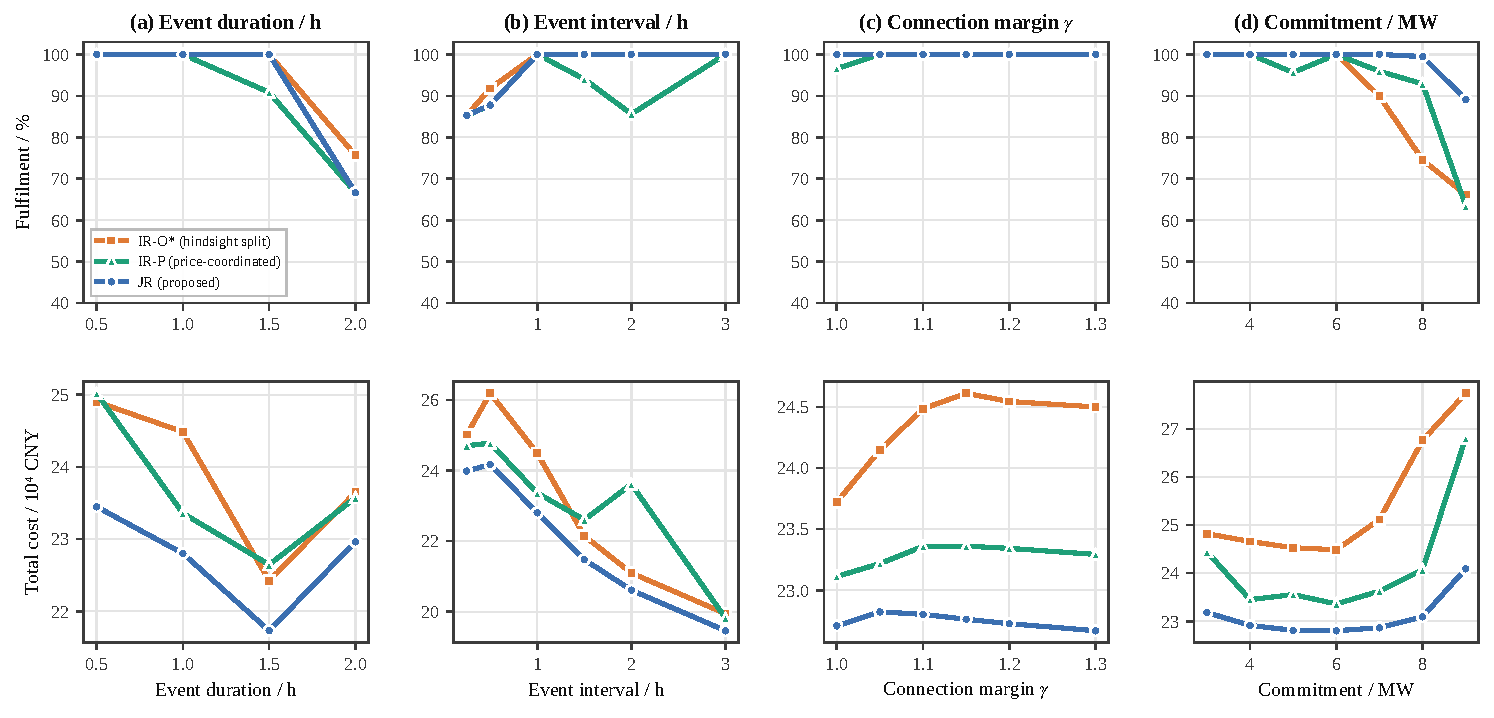
\includegraphics[width=0.96\textwidth]{fig05_sensitivity.pdf}
\caption{Sensitivity under perfect information ($\crb=3$~CNY/kW): fulfilment (top) and total cost (bottom) versus (a)
event duration, (b) event gap, (c) connection margin and (d) uniform commitment. The rule setting is shown in
\figref{fig:sens0}.}
\label{fig:sens}
\end{figure*}

\begin{figure*}[!t]
\centering
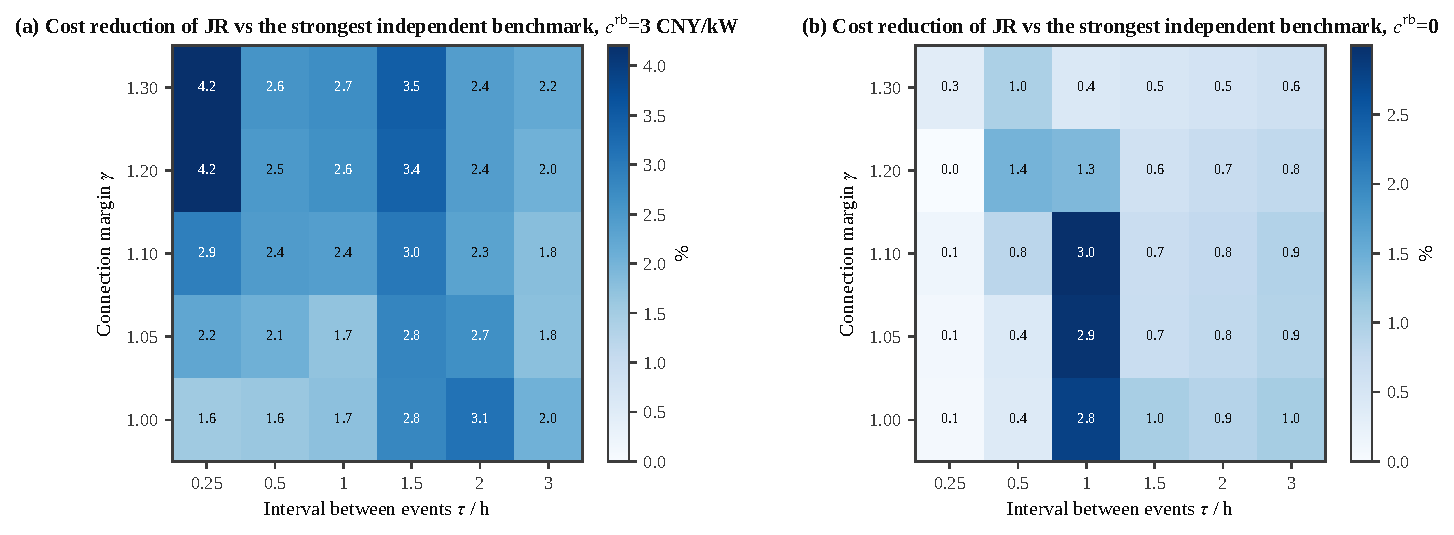
\includegraphics[width=0.94\textwidth]{fig06_interval_capacity_map.pdf}
\caption{Cost reduction of JR relative to the stronger of IR-O* and IR-P on the gap--margin plane: (a) rebound-priced
setting, (b) rule setting.}
\label{fig:map}
\end{figure*}

Deliverable capacity is the main value of joint recovery. With the requirement of $\ge$99\% fulfilment, even
hindsight-tuned independent recovery can commit only about 6~MW per event, whereas JR can commit about 8~MW (+33\%); at
8~MW, JR fulfils 99.5\% against less than 80\% for the best benchmark in the rule setting, at a 14.1\% lower cost. With
moderate commitments (6~MW) the advantage is only 2--3\%. On the gap--margin plane the reduction in the rule setting is
0--3.0\%, with the peak at a gap of 1~h and $\gamma\le1.10$ (2.8--3.0\%) and generally at most 1.4\% for gaps of 0.5~h
or less or 1.5~h or more; in the rebound-priced setting it is 1.6--4.2\% and never negative. Corollary~\ref{cor:novalue}
explains why the advantage first rises and then falls with the channel width: with a too narrow channel neither strategy
recovers, with a wide one both do.

Fulfilment is not what joint recovery maximises. With a gap of 0.5~h and $\crb=3$, JR fulfils 4--6 points less than
IR-O* but at a lower cost: the optimum delivers slightly above the 80\% validity threshold in some events to reduce the
rebound charge. With 2-h events, all three methods keep only two events valid. Both effects are cross-event trade-offs
induced by the Jiangsu settlement (80\% threshold, 120\% cap). Correcting the IT budget of the benchmarks
(\secref{sec:strategies}) has little effect under perfect information: at 6~MW the costs of IR-O* and IR-P drop by only
$0.06$--$0.07\times10^4$~CNY and the capacity conclusions are unchanged; the correction matters mainly for closed-loop
operation on heavy-load days.

\subsubsection{Rebound charge and DR payment}
\label{sec:sens-rebound}

\tabref{tab:rebound} and \figref{fig:rebound} treat the rebound charge as a policy parameter (case day, uniform 6~MW,
deterministic rolling operation). As the charge rises, the maximum rebound of JR-D after the events falls smoothly from
6.52 to 2.98~MW, its fulfilment stays at 100\% up to 4~CNY/kW, and JR-D is the cheapest strategy at every charge. IR-P
cuts the rebound to 2.04~MW at 6~CNY/kW, but its fulfilment drops to 65.9\%. On the plane of cost (excluding the rebound
charge) against maximum rebound, the trade-off curve of JR-D lies to the lower left of the benchmarks
(\figref{fig:rebound}(a)): controlling the rebound while keeping the events valid requires a joint allocation of the
channel. Without a rebound charge, however, joint recovery does not suppress the rebound by itself, since all strategies
raise the import to near the connection limit; whether and at which price to charge rebound is a policy choice of the
grid operator or aggregator, and joint recovery minimises its cost.

\begin{table}[!t]
\caption{Rebound charge as a policy parameter (case day, uniform 6~MW).}
\label{tab:rebound}
\centering\footnotesize
\setlength{\tabcolsep}{3pt}
\begin{tabular}{@{}lccccccc@{}}
\toprule
$\crb$ (CNY/kW) & 0 & 0.5 & 1 & 2 & 3 & 4 & 6\\
\midrule
JR-D max rebound (MW) & 6.52 & 6.47 & 6.45 & 6.31 & 5.77 & 5.27 & 2.98\\
JR-D cost ($10^4$~CNY) & 19.34 & 20.12 & 20.83 & 22.02 & 22.84 & 23.47 & 24.47\\
Best benchmark ($10^4$~CNY) & 19.97 & 20.79 & 21.57 & 22.60 & 23.61 & 24.48 & 25.88\\
& \scriptsize IR-O* & \scriptsize IR-O* & \scriptsize IR-O* & \scriptsize IR-P & \scriptsize IR-P & \scriptsize IR-P & \scriptsize IR-P\\
JR-D vs best & $-3.2\%$ & $-3.3\%$ & $-3.4\%$ & $-2.6\%$ & $-3.3\%$ & $-4.1\%$ & $-5.5\%$\\
\bottomrule
\end{tabular}
\end{table}

\begin{figure*}[!t]
\centering
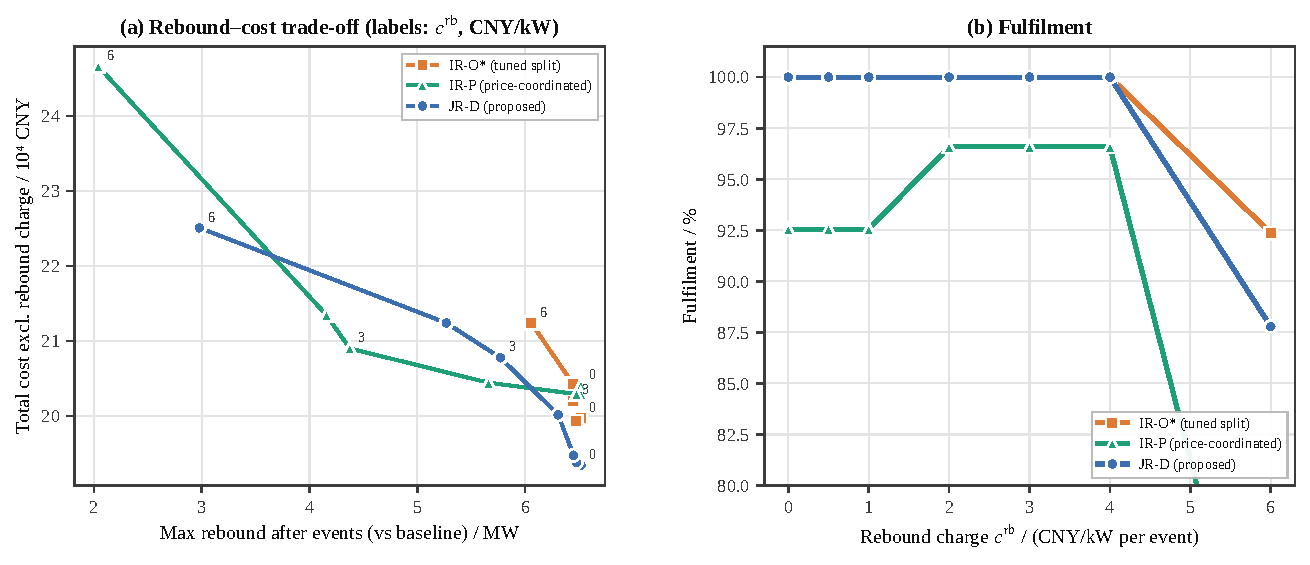
\includegraphics[width=0.84\textwidth]{fig10_rebound_pareto.pdf}
\caption{Rebound charge as a policy parameter. (a) Trade-off between the cost excluding the rebound charge and the
maximum rebound (labels: $\crb$ in CNY/kW); (b) fulfilment versus the rebound charge.}
\label{fig:rebound}
\end{figure*}

Across the nine combinations of DR payment (1--3~CNY/kWh) and shortfall coefficient ($\kappa$ = 0.5--2), JR-D is
always the cheapest, by 1.5\% (1~CNY/kWh, $\kappa=0.5$) to 4.0\% (3~CNY/kWh, $\kappa=2$) against the strongest benchmark
(\figref{fig:robust}(a)): the higher the payment and the stricter the shortfall assessment, the more valuable joint
recovery. At 1~CNY/kWh all three optimised strategies respond only partially (JR-D fulfils 33--88\%), since keeping
most events valid is no longer worthwhile.

\begin{figure*}[!t]
\centering
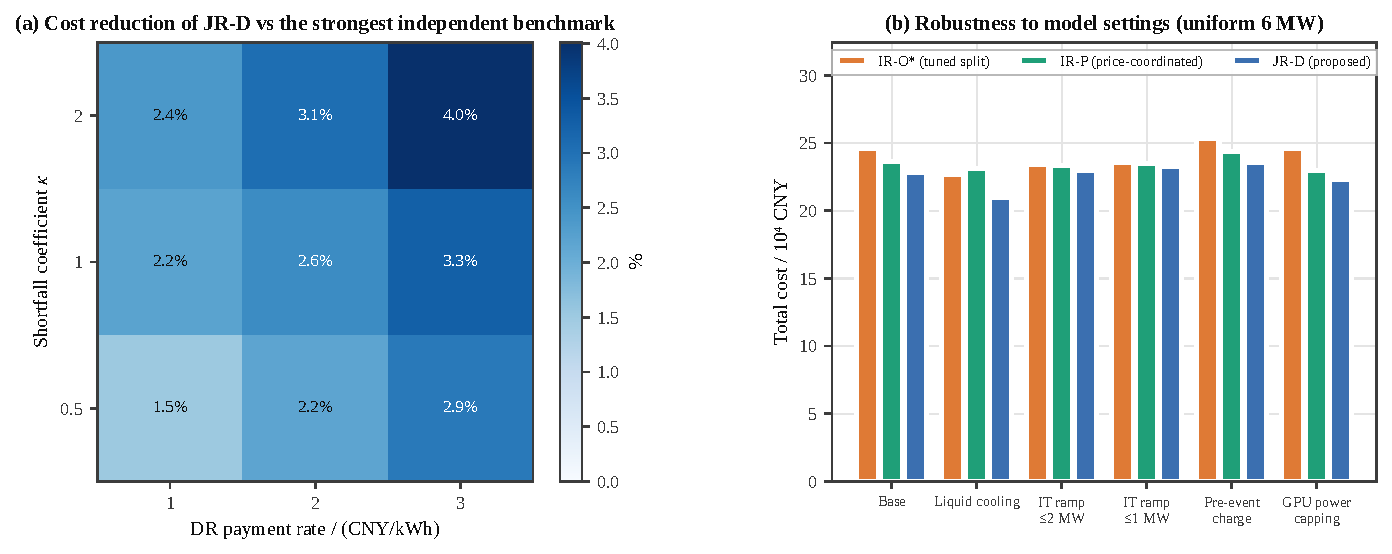
\includegraphics[width=0.90\textwidth]{fig13_robustness.pdf}
\caption{(a) Cost reduction of JR-D relative to the strongest independent benchmark for different DR payments and
shortfall coefficients; (b) total cost under different model settings (uniform 6~MW).}
\label{fig:robust}
\end{figure*}

\subsubsection{Realism, multi-energy coupling and policy constraints}
\label{sec:sens-real}

\tabref{tab:realism} and \figref{fig:robust}(b) add realistic features one at a time (uniform 6~MW, $\crb=3$,
deterministic rolling operation). Liquid cooling makes joint recovery more important: it lowers the cooling power, so the
connection limit, which follows the typical-day peak, falls to 14.59~MW and the channel narrows; IR-P then fulfils only
80.8\%, while JR-D still fulfils every event at a 7.4\% lower cost. IT ramp limits compress the room for joint recovery:
at 1~MW per 15~min the advantage shrinks to 0.8\%, because the ramp limit flattens the catch-up profile. A pre-event
load-up charge of 1,000~CNY/MWh adds the same amount to all strategies and does not change the schedule, since the
load-up stems from reserving storage for the events rather than from inflating the baseline. GPU power capping is an
effective additional lever: each unit of power reduction leaves only 0.4 units of debt, which lowers the cost of JR-D by
a further 2.4\% and its maximum rebound from 5.77 to 4.02~MW.

\begin{table}[!t]
\caption{Realism (uniform 6~MW, $\crb=3$): fulfilment / total cost ($10^4$~CNY).}
\label{tab:realism}
\centering\footnotesize
\setlength{\tabcolsep}{2.6pt}
\begin{tabular}{@{}lcccc@{}}
\toprule
Setting & IR-O* & IR-P & \textbf{JR-D} & JR-D vs best\\
\midrule
Base & 100\% / 24.57 & 96.6\% / 23.61 & \textbf{100\% / 22.84} & $-3.3\%$\\
Liquid cooling & 94.3\% / 22.66 & 80.8\% / 23.10 & \textbf{100\% / 20.98} & $-7.4\%$\\
IT ramp $\le$2~MW/15~min & 100\% / 23.45 & 98.1\% / 23.37 & \textbf{100\% / 22.98} & $-1.6\%$\\
IT ramp $\le$1~MW/15~min & 100\% / 23.56 & 95.5\% / 23.47 & \textbf{100\% / 23.29} & $-0.8\%$\\
Pre-event charge & 100\% / 25.31 & 96.6\% / 24.36 & \textbf{100\% / 23.59} & $-3.2\%$\\
GPU power capping & 92.0\% / 24.63 & 96.4\% / 22.94 & \textbf{100\% / 22.28} & $-2.9\%$\\
\bottomrule
\end{tabular}
\end{table}

\begin{figure*}[!t]
\centering
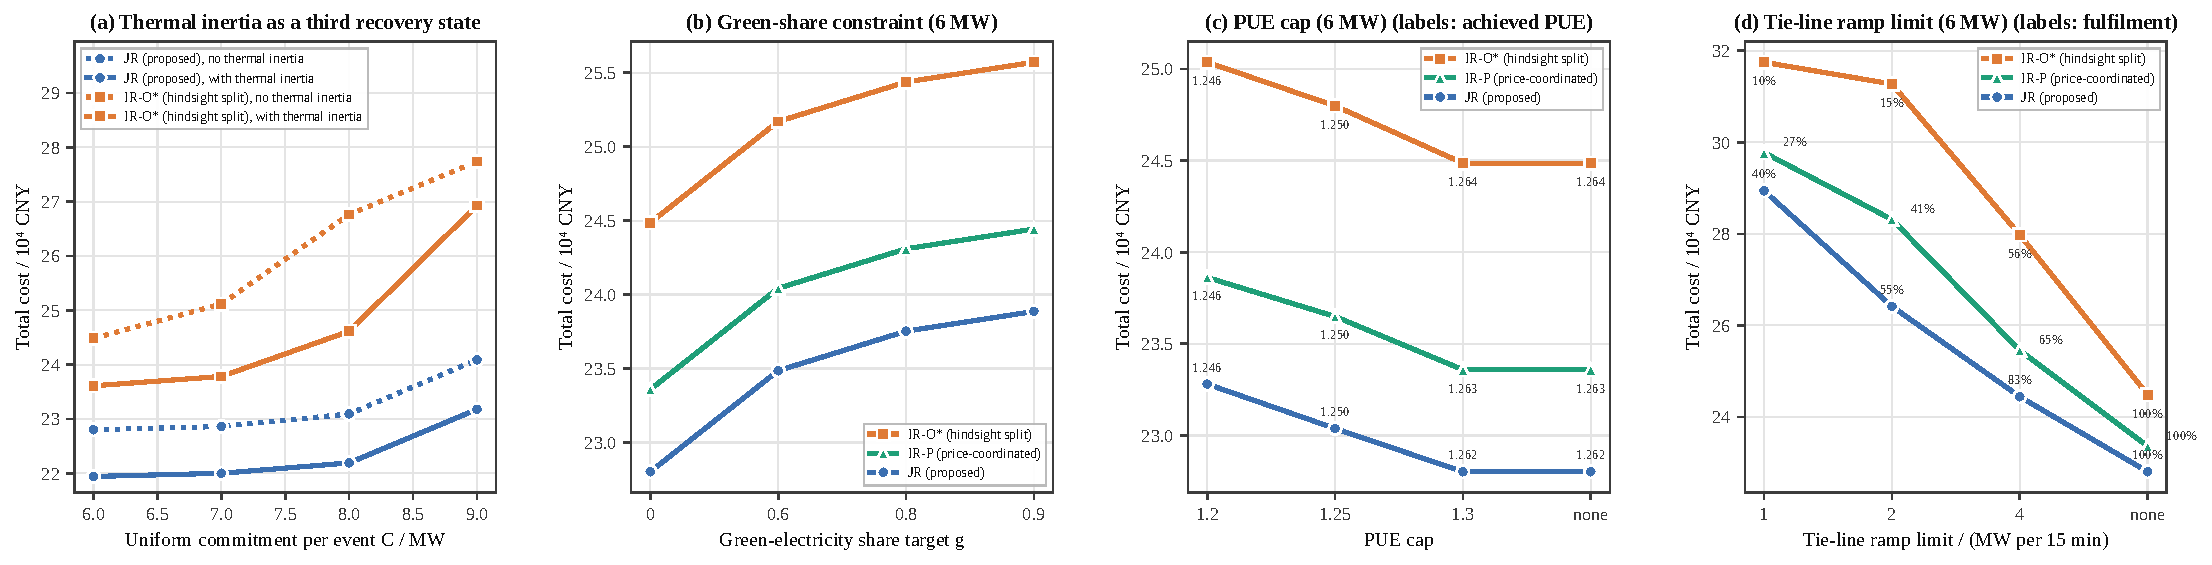
\includegraphics[width=\textwidth]{fig21_policy.pdf}
\caption{Multi-energy coupling and policy constraints ($\crb=3$, perfect information). (a) Data hall thermal inertia on
and off versus the commitment; (b) green-electricity share target; (c) PUE cap (labels: achieved PUE); (d) tie-line
ramp limit (labels: fulfilment).}
\label{fig:policy}
\end{figure*}

\figref{fig:policy} adds multi-energy coupling and policy constraints. Data hall thermal inertia acts as a third
recovery state: allowing the hall to float between $-2$ and $+3$~K around the set-point, all strategies use the full
3.0~K and save 0.86--0.88$\times10^4$~CNY per day (JR: 22.80 to 21.94), and in closed loop on 26 days JR-D saves 3.8\%
and IR-P 4.3\%. Thermal inertia is another free and fast storage that the facility side can use under independent
recovery too: at 8~MW the fulfilment of IR-P rises from 92.9\% to 99.4\%, level with JR (99.5\%). The advantage of joint
recovery remains but shrinks ($-2.6\%$ under perfect information at 8~MW, $-2.2\%$ in closed loop with
$p=1.5\times10^{-7}$), because more storage-side flexibility partly substitutes for joint recovery, as with large
batteries in \secref{sec:res-capacity}. Green-electricity targets of 60/80/90\% raise the daily cost of all strategies
by 0.68/0.95/1.08$\times10^4$~CNY with differences below 10~CNY between them, \ie\ in this accounting a green share acts
like a uniform surcharge on grid and gas electricity and does not change the ranking. Without a PUE cap, the PUE on the
DR day is 1.262--1.264; a cap of 1.25 is met by all strategies at an extra cost of 0.24 (JR) to 0.31 (IR-O*)
$\times10^4$~CNY by more absorption cooling, night-time TES charging and catch-up in cooler hours, whereas a cap of
1.20 is infeasible on this hot day (the minimum is 1.246, at 0.48--0.55$\times10^4$~CNY). Tie-line ramp limits of 4/2/1~MW
per 15~min directly restrict a fast load drop at the start of an event: the fulfilment of JR falls to
82.9/54.6/40.2\%, that of the benchmarks more (IR-P 64.9/41.2/27.2\%), and JR is 4.0/6.7/2.8\% cheaper than IR-P.
Without the limit, the largest step change of JR is a drop of 8.8~MW and a rise of 12.4~MW; since the Jiangsu rules judge
validity by the hourly mean, such ramp requirements would have to be designed together with the validity rule.

\subsubsection{Tariff shapes, seasons and climates}
\label{sec:sens-gen}

Five TOU shapes with the same daily mean are compared on 20 operating days (\figref{fig:gen}(a), \tabref{tab:tariff}).
The advantage of joint recovery is almost independent of the tariff shape: the cost reduction against IR-P is
2.1--2.9\% ($p\le4\times10^{-6}$), and the fulfilment of JR at 8~MW under perfect information is 99.5\% for every shape.
It is smallest under a flat tariff, where it matters less to which hours catch-up and recharging are moved.

\begin{table}[!t]
\caption{Tariff shapes (same daily mean): mean cost on 20 days ($10^4$~CNY) and fulfilment at 8~MW.}
\label{tab:tariff}
\centering\footnotesize
\setlength{\tabcolsep}{2.6pt}
\begin{tabular}{@{}lccc@{}}
\toprule
Tariff shape & \makecell{IR-O* / IR-P / JR-D} & \makecell{JR-D vs IR-P\\(paired)} & \makecell{8-MW fulfilment\\IR-O* / IR-P / JR}\\
\midrule
Jiangsu TOU (base) & 24.21 / 23.09 / 22.43 & $-2.86\%$ & 74.5 / 92.9 / 99.5\%\\
Flat & 27.94 / 27.08 / 26.51 & $-2.11\%$ & 74.5 / 93.0 / 99.5\%\\
Two-tier (peak 8--22~h) & 24.94 / 24.03 / 23.40 & $-2.61\%$ & 75.5 / 93.0 / 99.5\%\\
Critical peak (19--21~h) & 24.13 / 22.96 / 22.30 & $-2.85\%$ & 76.4 / 92.9 / 99.5\%\\
Duck curve & 25.20 / 24.22 / 23.53 & $-2.84\%$ & 69.3 / 92.9 / 99.5\%\\
\bottomrule
\end{tabular}
\end{table}

\begin{figure*}[!t]
\centering
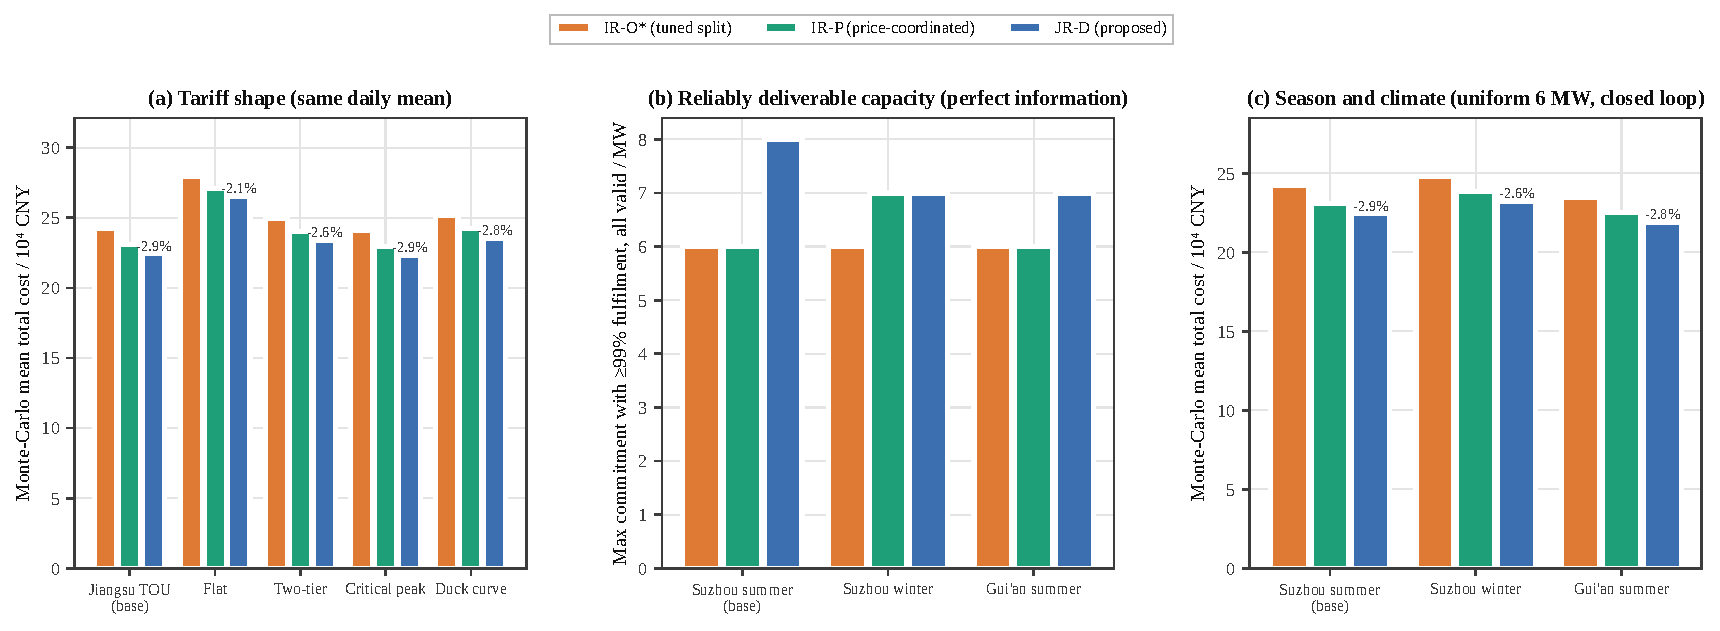
\includegraphics[width=0.98\textwidth]{fig20_generalization.pdf}
\caption{Generalisation. (a) TOU tariff shapes with the same daily mean (labels: JR-D relative to the stronger
benchmark); (b) reliably deliverable capacity under perfect information and (c) closed-loop mean cost for three climates.}
\label{fig:gen}
\end{figure*}

\begin{table}[!t]
\caption{Seasons and climates (same computing traces, Jiangsu rules and tariff).}
\label{tab:climate}
\centering\footnotesize
\setlength{\tabcolsep}{2.4pt}
\begin{tabular}{@{}lcccccc@{}}
\toprule
Case & \makecell{$\Pcap$\\(MW)} & \makecell{Mean\\COP} & \makecell{PV\\(MWh/d)} & \makecell{Reliable cap.\\IR-O*/IR-P/JR\\(MW)} & \makecell{All valid\\IR-O*/IR-P/\\JR-D} & \makecell{JR-D\\vs IR-P}\\
\midrule
\makecell[l]{Suzhou\\summer} & 16.03 & 5.13 & 38.9 & 6 / 6 / \textbf{8} & 90 / 95 / \textbf{100\%} & $-2.86\%$\\
\makecell[l]{Suzhou\\winter} & 15.51 & 7.00 & 26.0 & 6 / 7 / \textbf{7} & 95 / 95 / \textbf{100\%} & $-2.61\%$\\
\makecell[l]{Gui'an\\summer} & 15.67 & 5.77 & 44.9 & 6 / 6 / \textbf{7} & 95 / 95 / \textbf{100\%} & $-2.80\%$\\
\bottomrule
\multicolumn{7}{@{}p{0.97\columnwidth}@{}}{\scriptsize Reliable capacity under perfect information ($\ge$99\% fulfilment, all events valid); closed loop on 20 days at 6~MW, paired $p=4\times10^{-6}$ in all cases.}
\end{tabular}
\end{table}

Three climates use the same computing traces, Jiangsu rules and tariff: summer in Suzhou (base, maximum 38.3~$^\circ$C),
winter in Suzhou (10 January 2025, minimum $-3.0~^\circ$C) and summer in Gui'an (26 July 2024, maximum 31.7~$^\circ$C), a
national computing hub (\tabref{tab:climate}). In all three, JR-D keeps every event valid on every day and costs about
2.6--2.9\% less than IR-P. In winter and in the cooler climate the cooling load is lower and the COP higher, so less
cooling-related electricity can be shifted and the reliable capacity of JR drops to 7~MW; in winter IR-P also reaches
7~MW. The value of joint recovery thus follows the scarcity of the recovery channel, as Theorem~\ref{thm:closed}
predicts, and is largest in the evening peak of hot summer days. The coincidence of the drivers explains why that peak is
tight (\figref{fig:drivers}): in normal operation the storage discharges in the peak-price hours, which lowers the
17:00--22:00 baseline to about 9.6~MW, and PV has vanished while the price is still high, so reductions must rely more
on deferring computing and extra storage discharge, and the subsequent recovery need is larger.
